\begin{frame}[t]\frametitle{Backtest Study - 2}\bigskip
	We present an application for Algorithm~InexProj-SGM, a backtest study of a portfolio build with the \textcolor{purple}{5 most volatile brazilian companies} of 2016: Gerdau S.A. (GGBR4, GOAU4), CSN S.A (CSNA3), RUMO S.A. (RAIL3), Usiminas (USIM5) and the \textcolor{purple}{5 least volatile assets} of 2016: Ambev S.A. (ABEV3), Engie S.A. (EGIE3), Ultrapar S.A. (UGPA3), Equatorial (EQTL3), Raia Drogasil S.A. (RADL3).

	 We did a backtest, building 2 portfolios with monthly rebalance:
	 \begin{itemize}
	 	\item One was the minimum variance portfolio (MVP), 
	 	\item the other the risk parity portfolio (RPP).
	 \end{itemize}

	 Data pertaining to the period between January 2016  and June 2022, was taken from Yahoo Finance (\url{http://finance.yahoo.com}). For rebalancing, the volatilities were calculated using data from the previous 12 months. 2016 year data was used only for past volatilities calculations.
\end{frame}



\begin{frame}[t]\frametitle{}
	\begin{figure}[H]
		\begin{adjustwidth}{1cm}{1cm}
			\begin{subfigmatrix}{2}
				\subfigure[Weigths]{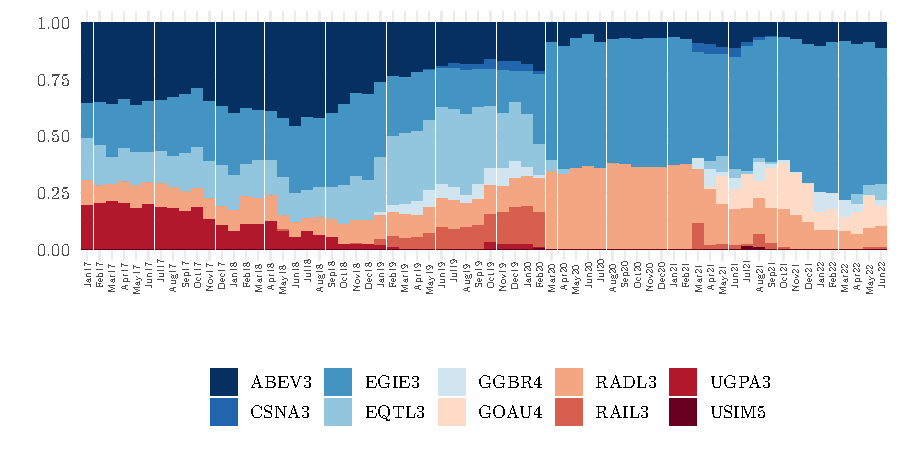
\includegraphics{../figures/WeigthMVPvolHighLow.pdf}}
				\subfigure[Risks]{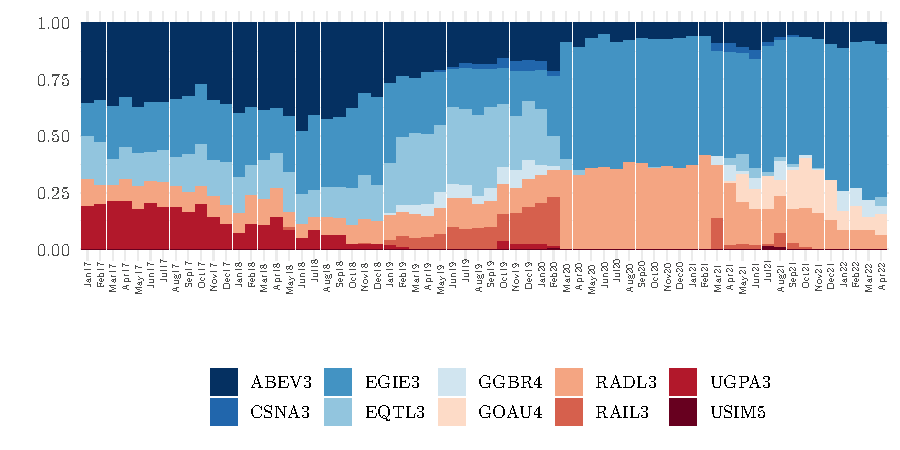
\includegraphics{../figures/RiskMVPvolHighLow.pdf}}
			\end{subfigmatrix}
			\caption{Monthly distribution of MVP.}
			\label{fig:totalRiskMVP}
		\end{adjustwidth}
	\end{figure}


	\begin{figure}[H]
		\begin{adjustwidth}{1cm}{1cm}
			\begin{subfigmatrix}{2}
				\subfigure[Weigths]{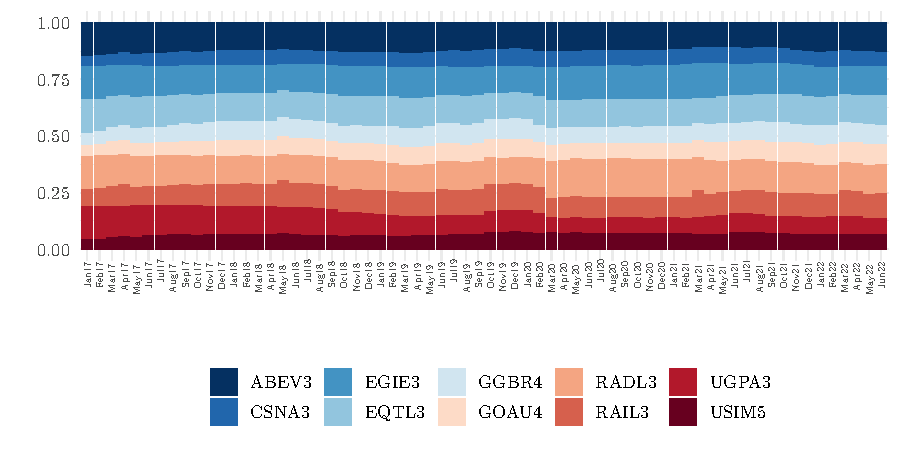
\includegraphics{../figures/WeigthRPPvolHighLow.pdf}}
				\subfigure[Risks]{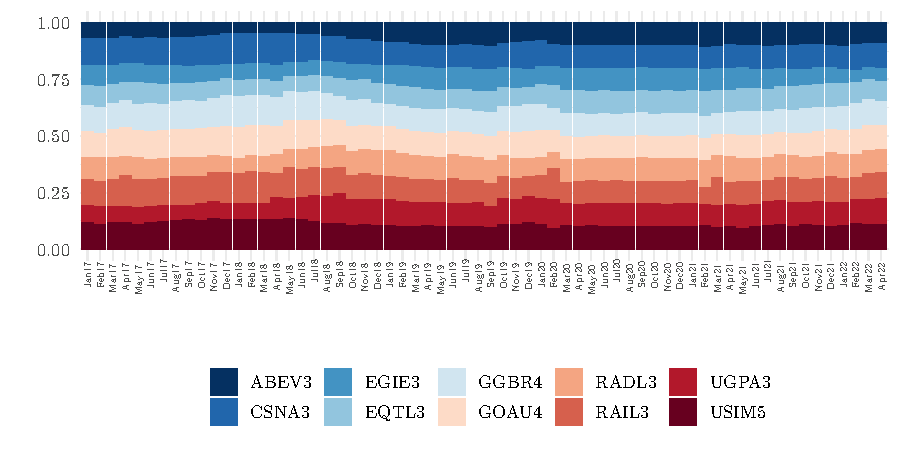
\includegraphics{../figures/RiskRPPvolHighLow.pdf}}
			\end{subfigmatrix}
			\caption{Monthly distribution of RPP.}
			\label{fig:totalRiskPPP}
		\end{adjustwidth}
	\end{figure}
\end{frame}

\begin{frame}[t]\frametitle{}\bigskip

	\begin{figure}[H]
		\centering
		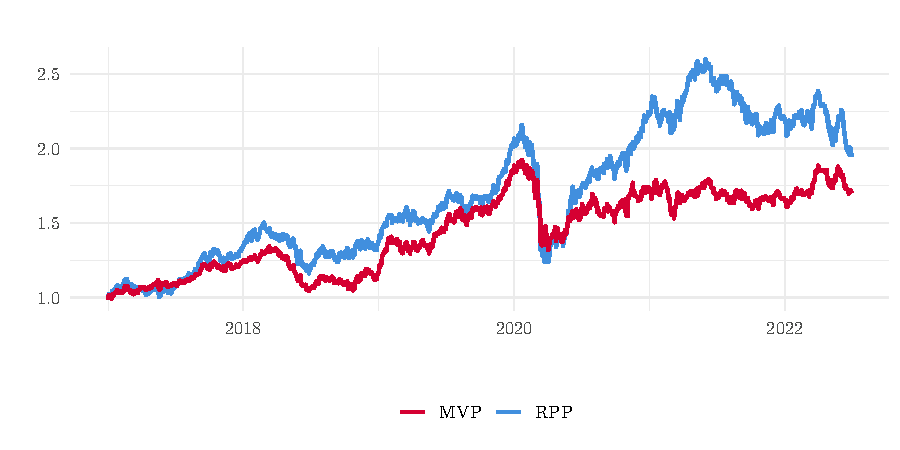
\includegraphics[width=0.7\linewidth]{../figures/retornovolHighLow.pdf}
		\caption{MVP and RPP accumulated returns: January 2017 $-$ June 2022.}
		\label{fig:retornoRPPMVP}
	\end{figure}


	\begin{table}[!htb]
	\centering
	\begingroup
	\fontsize{9}{9}
	\selectfont
	\begin{tabular}{lrr}
		\toprule
		                                    & MVP    & RPP    \\
		\midrule
		\textbf{Annualized Return}          & 0.1035 & 0.1317 \\
		\textbf{Annualized Std Dev}         & 0.2122 & 0.2552 \\
		\textbf{Annualized Sharpe (Rf=0\%)} & 0.4880 & 0.5160 \\
		\bottomrule
	\end{tabular} \caption{Annualized Returns: Jan17 - Jun22}
	\label{tab: volHighLow }
	\endgroup{}
\end{table}

\end{frame}

\begin{frame}[t]\frametitle{}\bigskip

	\begin{figure}[H]
		%\begin{adjustwidth}{2.2cm}{2.2cm}
		\begin{subfigmatrix}{2}
			\subfigure[January 2017 $-$ December 2019.]{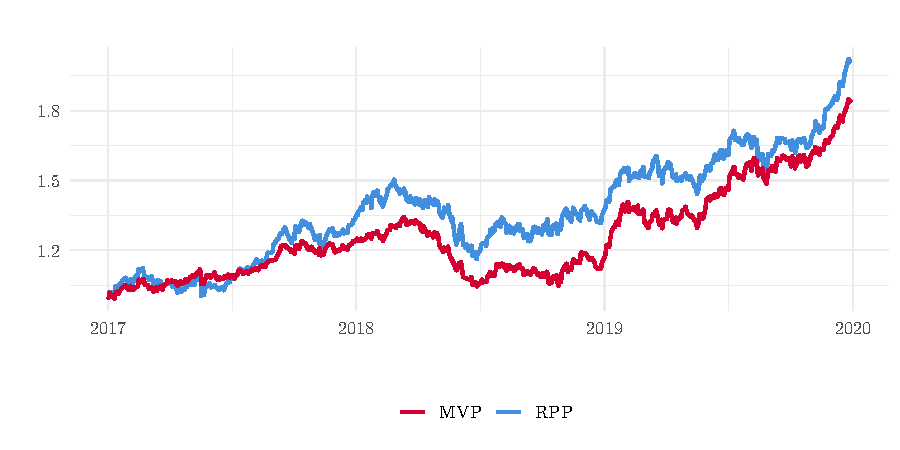
\includegraphics{../figures/retornovolHighLow1.pdf}}
			\subfigure[January 2020 $-$ June 2022.]{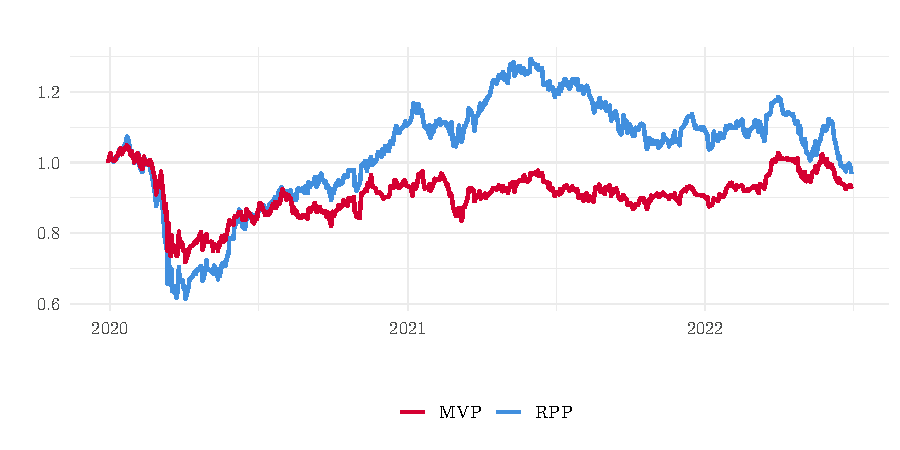
\includegraphics{../figures/retornovolHighLow2.pdf}}
		\end{subfigmatrix}
		\caption{MVP and RPP accumulated returns.}
	%	\label{fig:retornoRPPMVP12}
		%\end{adjustwidth}
	\end{figure}

{}
	\begin{table}[!htb]
		% \caption{Global caption}
		\begin{minipage}{.5\linewidth}
		
\begin{tabular}{lrr}
	\toprule
	                                    & MVP    & RPP    \\
	\midrule
	\textbf{Annualized Return}          & 0.2298 & 0.2688 \\
	\textbf{Annualized Std Dev}         & 0.1590 & 0.1943 \\
	\textbf{Annualized Sharpe (Rf=0\%)} & 1.4447 & 1.3836 \\
	\bottomrule
\end{tabular} \caption{Jan17 - Dez19}

			% \begin{table}[!htb]
			% 	\centering
			% 	\begingroup
			% 	\fontsize{7}{7}
			% 	\selectfont
			% 	\begin{tabular}{>{}lrr}
			% 		\toprule
			% 		                                    & MVP    & RPP    \\
			% 		\midrule
			% 		\textbf{Annualized Return}          & 0.2107 & 0.3212 \\
			% 		\textbf{Annualized Std Dev}         & 0.1744 & 0.2027 \\
			% 		\textbf{Annualized Sharpe (Rf=0\%)} & 1.2087 & 1.5851 \\
			% 		\bottomrule
			% 	\end{tabular} \caption{January 2017 - December 2019.}
			% %	\label{tab:RPP1}  % LEMBRE-SE DE MUDAR O LABEL
			% 	\endgroup{}
			% \end{table}
		\end{minipage}%
		\begin{minipage}{.5\linewidth}
		
\begin{tabular}{lrr}
	\toprule
	                                    & MVP     & RPP     \\
	\midrule
	\textbf{Annualized Return}          & -0.0305 & -0.0130 \\
	\textbf{Annualized Std Dev}         & 0.2619  & 0.3128  \\
	\textbf{Annualized Sharpe (Rf=0\%)} & -0.1165 & -0.0415 \\
	\bottomrule
\end{tabular} \caption{Jan20 - Jun22}
			% \begin{table}[!htb]
			% 	\centering
			% 	\begingroup
			% 	\fontsize{7}{7}
			% 	\selectfont
			% 	\begin{tabular}{>{}lrr}
			% 		\toprule
			% 		                                    & MVP     & RPP     \\
			% 		\midrule
			% 		\textbf{Annualized Return}          & -0.0631 & -0.0278 \\
			% 		\textbf{Annualized Std Dev}         & 0.3046  & 0.3227  \\
			% 		\textbf{Annualized Sharpe (Rf=0\%)} & -0.2070 & -0.0860 \\
			% 		\bottomrule
			% 	\end{tabular}
			% 	\caption{January 2020 - June 2022.}
			% %	\label{tab:RPP2}  % LEMBRE-SE DE MUDAR O LABEL
			% 	\endgroup{}
			% \end{table}
		\end{minipage}
	\end{table}
\end{frame}